\chapter{Results}
This section is divided into multiple sub-sections; each part explains the different aspects of our research.

\section{Training Time Cost}
As mentioned earlier, the computational cost for DTM is higher than LDA;  however, to determine the difference in training time, we conducted a small sub-experiment in which we trained both the DTM and LDA models with different-size documents and hyperparameter value $K$, which is the number of topics. The dataset used for this experiment was the "Twitter" dataset. Preprocessing cleaning and hashtag pooling were applied before training.

\begin{figure}[h!]
\begin{center}
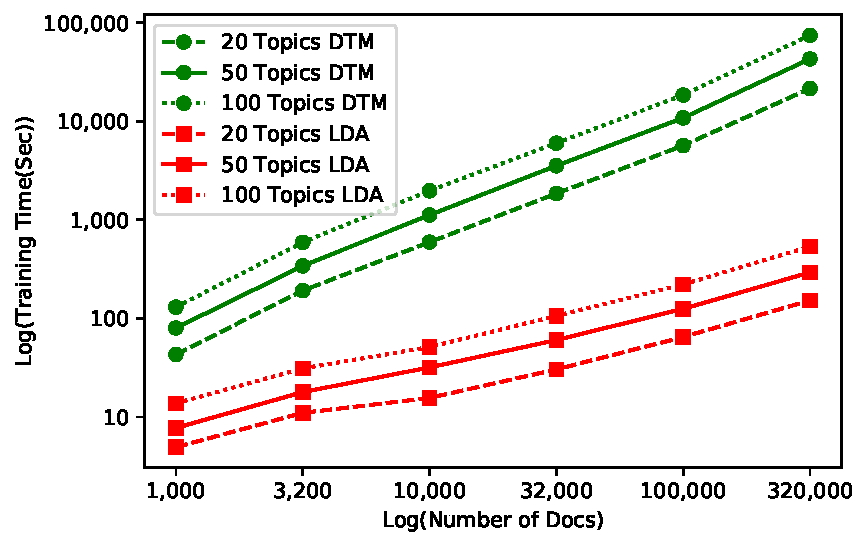
\includegraphics[scale=0.8]{costGraph.pdf}
\caption{This graph is in logarithmic scale to fit higher values into the figure. The x-labels are the number of documents on which the models were trained and y-axis is the time in seconds that each model took for training.}
\label{fig:trainingTime}
\end{center}
\end{figure}

\textbf{Figure \ref{fig:trainingTime}} shows that increasing the number of documents or the number of topics increase the training time. We see a roughly linear increase in time for both models. For small datasets, the training time of DTM was 10 times more than LDA and exceeds \textbf{"100 times"} for big datasets. Normally in NLP topic modeling problems, datasets are relatively bigger in size. We can therefore say that DTM will take around 100 times more time for training compared with LDA under the same conditions.

\section{Topic Drifting}
Topic drifting is fundamental information extracted from DTM. A single DTM topic consists of topics at each time slot. For clarity, let us call such a time-slice-topic the "focus" of the DTM topic. The focus of a DTM topic changes over time, as shown in the first part of \textbf{Figure \ref{fig:fragmentation}}, where the focus changed from "Signal Processing" to "Tensor Decomposition" by the end. This is called topic drifting or topic transition. We calculated the total unique vocabularies for each DTM topic. The minimum vocabulary size for any topic was 50. If any topic had $V_s$ close to this number, it means there were no new words in the different time slot topics. In short, the focus of this specific topic remained the same and there was no topic drifting.

\begin{table}[h!]
\begin{center}
\begin{tabular}{|c|c|c|c|c|}
\hline \textbf{Dataset} & \textbf{Topics} & $K(V_s > 70)$& $K(V_s > 90)$ & $K(V_s > 120)$ \\ \hline

\multirow{3}{*}{NeurIPS}  & 30 & 13 & 8 & 0 \\ & 60 & 58 & 56 & 11  \\ & 90 & 90 & 90 & 90  \\ \hline
\multirow{3}{*}{Twitter}  & 30 & 3 & 1 & 0 \\ & 60 & 3 & 0 & 0 \\ & 90 & 1 & 0 & 0 \\ \hline
\multirow{3}{*}{News}  & 30 & 29 & 20 & 5 \\ & 60 & 57 & 33 & 1 \\ & 90 & 83 & 37 & 2 \\ \hline

\end{tabular}
\caption{$V_s$ is the vocabulary size, which is the number of unique words that appeared in all time slot topic-word distributions of a single DTM topic. Minimum $V_s$ is 50.  $K(V_s > 70)$ means the number of DTM topics having a vocabulary size of more than 70. Similarly $K(V_s > 90)$ and $K(V_s > 120)$ mean the number of topics having a vocabulary size of more than 90 and 120, respectively. }
\label{table:topicDrifting}
\end{center}
\end{table}

In \textbf{Table \ref{table:topicDrifting}}, $K(V_s)$ values for the Twitter dataset are very low, which means there were not many new words in the DTM topics and the focus of the topics remained the same over all times. This implies that DTM topic drifting for the Twitter dataset is negligible. And $K(V_s)$ values for the DTM trained on NeurIPS and News dataset were relatively high, which implies that there were topic drifting phenomenons.

\section{JS Analysis}
To extract the information overlap of the DTM and LDA topics, we computed JS values using \textbf{Equation 6} for all the datasets in all topic configurations. The JS value is bounded by 0 and 1 for two distributions, where 0 means both distributions are identical and 1 means there is no similarity between both probability distributions. A threshold value of 0.7 was selected and any DTM topic distribution having a JS value lower than or equal to this threshold when measured with the LDA topic distributions was part of the related topic "RT", Fragmented topic "FT", and others. A summary of this analysis is set forth in \textbf{Table \ref{table:JStable}}.

\begin{table}[h!]
\begin{center}
\begin{tabular}{|c|c|c|c|c|c|c|}
\hline \textbf{Dataset} & \textbf{Topics} & \textbf{RT}& \textbf{FT} & \textbf{F 2} & \textbf{F 3} & \textbf{F 4 \& more} \\ \hline

\multirow{3}{*}{NeurIPS}  & 30 & 17 & 4 & 3 & 1 & 0 \\ & \textbf{60} & \textbf{42} & \textbf{16} & \textbf{11} & \textbf{5} & 0  \\ & 90 & 69 & 28 & 25 & 2 & 1 \\ \hline
\multirow{3}{*}{Twitter}  & 30 & 5 & 0 & 0 & 0 & 0 \\ & 60 & 11 & 1 & 1 & 0 & 0 \\ & 90 & 14 & 3 & 2 & 1 & 0 \\ \hline
\multirow{3}{*}{News}  & 30 & 8 & 1 & 1 & 0 & 0 \\ & 60 & 24 & 2 & 2 & 0 & 0 \\ & 90 & 42 & 4 & 4 & 0 & 0 \\ \hline

\end{tabular}
\caption{DTM and LDA trained on "Dataset with "Topics" configuration one at a time, "RT" is the total number of DTM topics having a relationship with the LDA topic/s. "FT", "F2", "F 3", and "F 4 \& more" are the number of DTM topics having a JS relationship with two or more LDA topics, only two LDA topics, only three LDA topics, and more than three LDA topics, respectively.}
\label{table:JStable}
\end{center}
\end{table}

\textbf{Table \ref{table:JStable}} shows that a negligible amount of "FT" fragmented topics was found for the datasets "News" and Twitter" because most news articles and tweets are instantaneous responses of some events, and these topics die within short period of time; in other words, we see other tweets and article about other events. Due to this focus shifting behavior of the documents, DTM cannot accurately locate topic transitions over time. That is why very few fragmented topics were found for these datasets. Related topics "RT" are comparatively higher for "News" as compared to "Twitter" dataset because the domain of tweets is huge; it could be anything ranging from personal (My pet is very cute) to political (US president announced a restriction on trade agreement with China), whereas the News articles domain is restricted compared with Twitter. We can therefore have many topics in the Twitter dataset and random initial conditions of both DTM and LDA. It is safe to say that both models could come up with different topics. As mentioned,  the News dataset domain is restricted so we see high topic overlapping values in this dataset's results.

The domain of the "NeurIPS" documents focused on a few subjects(machine learning, artificial intelligence, computational neuroscience, etc.), so related topics' "RT" values are very high compared with other dataset configurations. High fragmented topic "FT" values can be seen for the "NeurIPS" dataset in \textbf{Table \ref{table:JStable}} because research papers tend to follow previous researches or somehow align with previous research papers. That is why we can see a well-defined topic transitions in the DTM topics, as shown in \textbf{Fig \ref{fig:fragmentation}}.

In all the datasets, increasing the number of topics resulted in an increase in "RT" and "FT" values.

\begin{table}[h!]
\begin{center}
\begin{tabular}{|c|c|c|c|c|c|c|c|}
\hline \textbf{Dataset} & \textbf{DTM} & \textbf{LDA} & \textbf{RT}& \textbf{FT} & \textbf{F 2} & \textbf{F 3} & \textbf{F 4 \& more} \\ \hline

NeurIPS & 30 & 1000 & 25 & 20 & 3 & 7 & 10 \\ \hline

\end{tabular}
\caption{A special configuration with DTM topics and LDA topics was also examined to analyze the behavior of an LDA model trained with a high number of topics.}
\label{table:JS30DTM1000LDA}
\end{center}
\end{table}

If we increase the number of topics in LDA, we get more and more fragmented topics, which means that topics are further divided into smaller and more focused themes. DTM's computation cost restricts us from increasing the number of topics, so we cannot get the type of topics that we can get from LDA with a very high $K$ hyperparameter.

\section{Overall Correlation}
Due to fragmentation detection, being part of a single DTM topic, fragmented LDA topics should have some relationship with each other. For example, the documents that have a high probability of topic 0 shown in \textbf{Figure \ref{fig:fragmentation}} in the DTM analysis should have a high probability for topic 19 and 55 in the LDA analysis as compared to other topics. This phenomenon leads to the hypothesis that \textit{"fragmented topics have similar distributions"}. Therefore we find the overall correlation coefficient for all the fragmented topics extracted from the LDA model trained on the "NeurIPS" dataset with $K = 60$.
After training the model, topic distribution for each document was calculated using the method described in \textbf{Section 3}. This topic distribution gives us insights into the relevance of each topic with each topic. Document-topic probabilities of the fragmented topics were used as variables to calculated the overall correlation.

The analysis showed no significant results and most of the correlation values were around 0, which means there is no linear relationship between fragmented topics, with few exceptions ranging up till "0.44" indicating some relation but not significant enough to prove our hypothesis.

\section{Time Series Correlation}
We also checked the correlation in a time-series manner because fragmented topics have time-series effects. For example \textbf{Figure \ref{fig:fragmentation}} shows that the JS similarity for both topics was close until the 15th time slot and the DTM topic was biased towards topic 19 as compared to topic 55 around the end. It is also, therefore, worth checking the relationship of fragmented topics in a time-series manner to further explore our hypothesis.

We split the document-topic distribution according to the time slots, checked the correlation of the fragmented topics in each time slot, and then made a graph to view the correspondence of the time-series correlation graph with JS graphs. The resultant graphs showed no strong relationship between fragmented topics and we could not find evidence to prove our hypothesis \textit{fragmented topics have similar distributions}.

\section{Time Series Topic Popularity}
Topic popularity is the second fundamental information that can be extracted from a topic model and, especially in the case of DTM, time-series topic popularity is estimating the number of documents for each topic at each time slice. We can easily construct this information into a self-explanatory graphical representation of topic popularity. For this analysis, we selected the 60 topics of the "NeurIPS" configuration. Then $\gamma$ distributions for the documents were calculated which gives the probability of each topic for each document. Time-depended summation over the topics then gives us the estimated number of documents for each topic at each time slot. we can also extract this information from LDA with just a few extra steps. First, we trained the LDA with the same dataset and got topics with the same 60-topic configuration. Before getting the $\theta_{dk}$ distributions for the documents, we saved the date information with the documents so that when we got the $\theta_{dk}$ distributions, we knew the corresponding date of each document. With these distributions and dates, we applied time-dependent summation over the topics and got an estimated number of documents for each topic at each time slot. Afterward, we plotted this information into graphs. To reduce noise effects and to make the graphs smooth, we used the Savitzky-Golay digital filter.

\begin{figure}[h!]
\begin{center}
\begin{tabular}{cc}
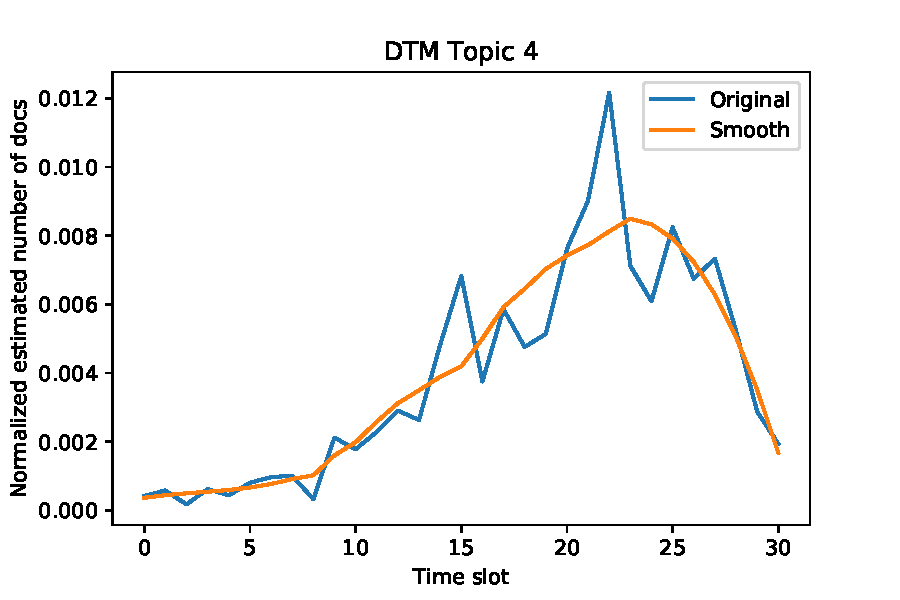
\includegraphics[scale=.5]{DTMpopulationTopic4.pdf} &
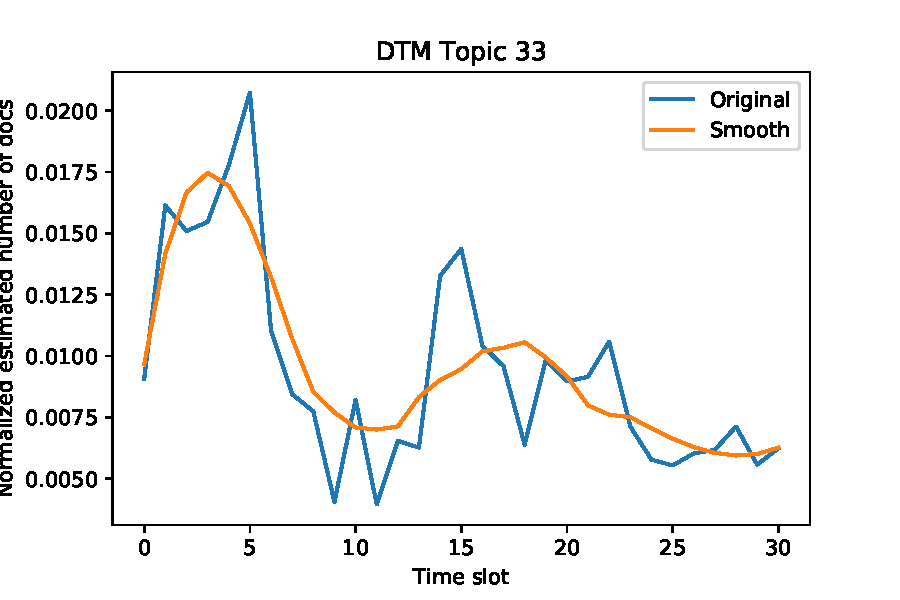
\includegraphics[scale=.5]{DTMpopulationTopic33.pdf} \\
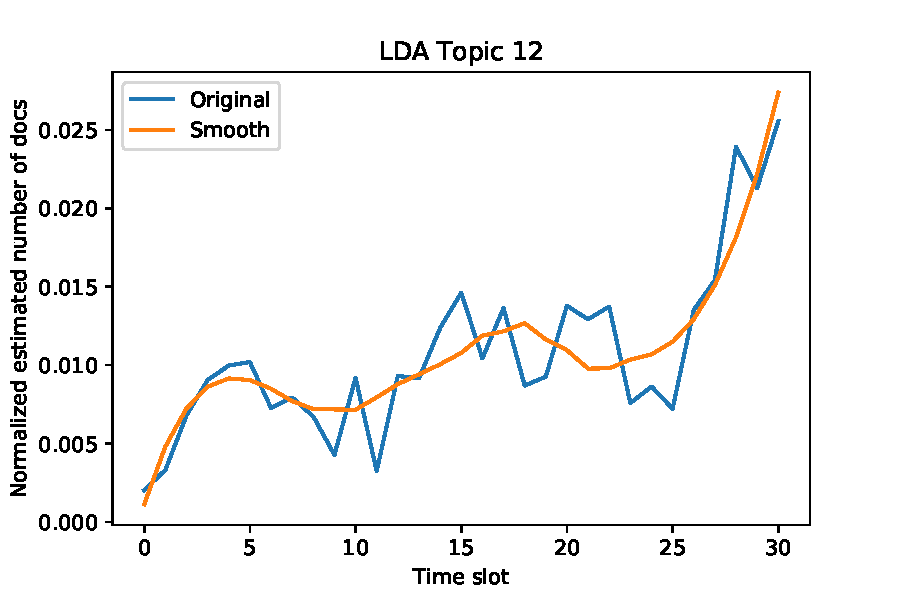
\includegraphics[scale=.5]{LDApopulationTopic12.pdf} &
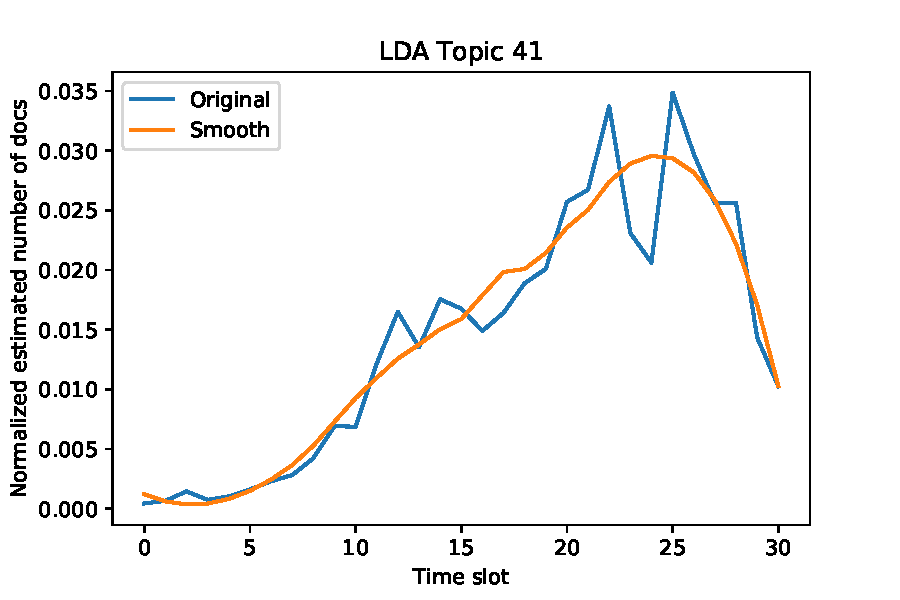
\includegraphics[scale=.5]{LDApopulationTopic41.pdf}
\end{tabular}
\caption{Number of documents for each time slot estimated from $\gamma$ and $\theta$ distributions of the documents for DTM and LDA respectively. Two topics from each model are shown here. The horizontal axis shows the time slot number and the vertical axis is the normalized estimated number of documents for these topics.}
\label{fig:populationGraphs}
\end{center}
\end{figure}


\textbf{Figure \ref{fig:populationGraphs}} shows the time-series topic popularity of both the DTM and LDA topics. The top two graphs in the figure are of DTM topics 4 and 33, respectively, and the bottom graphs show the time-series popularity of LDA topics 12 and 41. These graphs show that the time-series topic popularity can be extracted from DTM as well as LDA.
